\documentclass{article}
\usepackage{graphicx}
\usepackage[utf8]{vietnam}

\title{Labwork 4: Threads}
\author{Pham Quang Duong - 2540048}
\date{}

\begin{document}

\maketitle

\section{Implementation}

For this assginment, we implement the code grayscale CUDA from labwork 3 and improve it using 2D blocks with 2D grid. Each CUDA thread directly processes one image pixel using its $(x,y)$ coordinates, instead of using a 1D index.

\section{2D Block Size Experiment}

Different 2D block sizes were tested, including $(8,8)$, $(16,8)$, $(8,16)$, $(16,16)$, $(32,16)$, $(16,32)$, and $(32,32)$. We use time.time() fuction to measure execution time and we did a warm-up run before timing, and the reported execution time was calculated as the average of five runs.

The average execution time was between $0.00398$ seconds and $0.00903$ seconds. Compared to the older 1D method, which took much longer because of mapping delays, the 2D block design ran faster because it matched the image's shape. The best performance came from the $(32,16)$ block size, taking about $0.00398$ seconds.

\begin{center}
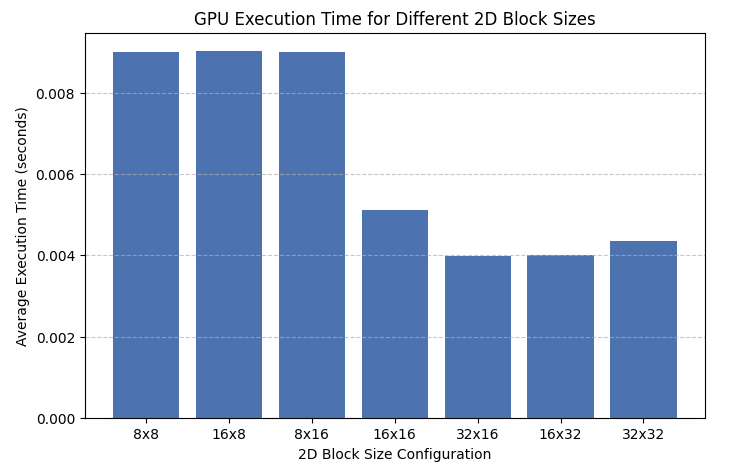
\includegraphics[width=0.8\textwidth]{execution_time.png}
\end{center}

\end{document}